\chapter{VisualHFSM 5.0}\label{chap:VisualHFSM5}
En este capítulo empezaremos comentando brevemente las características principales de la herramienta para poner en situación al lector. Después, describiremos la solución que hemos desarrollado para cumplir los objetivos y los requisitos previamente comentados. La idea es explicar en detalle todas las novedades que introduce VisualHFSM 5.0 y cómo se han llevado a cabo, terminando con las limitaciones que existían en su anterior versión. Para esto, hemos agrupado los cambios en distintas secciones. Primero, empezaremos comentando los cambios relacionados con el propio editor gráfico. Después comentaremos la GUI en ejecución para el componente de C++, para a continuación, hablar sobre la posibilidad de generar código en Python y la GUI en ejecución para estos componentes en Python, que aunque en apariencia es igual se ha realizado de forma distinta, utilizando otra librería gráfica. Por último, hablaremos de las medidas que hemos tomado para dar a conocer nuestra herramienta y facilitar que sea utilizada por terceros. \\

VisualHFSM cuenta con distintas partes bien diferenciadas, como se observa en la figura \ref{fig:partesVisualHFSM}. En primer lugar tiene el \emph{editor gráfico}, que permite crear el diagrama de estados y editar el comportamiento del robot. Todo el comportamiento generado con el editor se guarda en un \emph{archivo XML}, que se utiliza para poder retomar el proyecto más tarde. Además, cuenta con un \emph{generador de código}, que utiliza el archivo XML guardado mediante el editor gráfico y una \emph{plantilla} para generar el código del componente, el archivo de configuración de ICE y el archivo para la compilación de la aplicación, en caso de que sea necesario. En las aplicaciones en C++ el componente se genera al compilar el código fuente, que puede realizarse desde el editor gráfico también, y en las aplicaciones en Python el propio código se genera como un ejecutable, siendo el componente también. 

\begin{figure}[htbp]
	\centering
	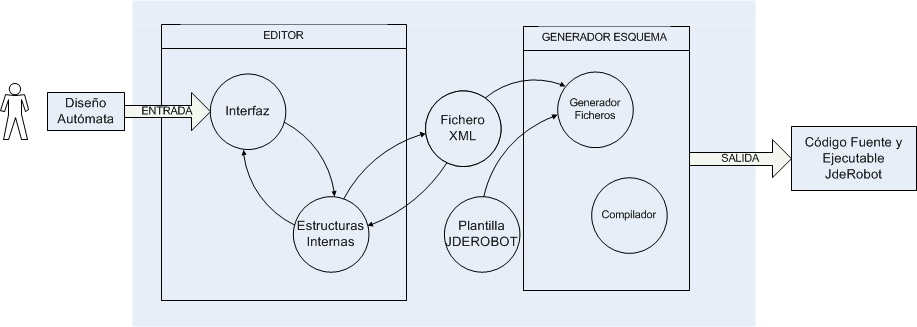
\includegraphics[height=5cm]{imgs/4_visualHFSM5/cajaBlanca.jpg}
	\caption{Esquema con los elementos de VisualHFSM}
	\label{fig:partesVisualHFSM}
\end{figure}


%%%%%%%%%% Mejoras en el editor gráfico %%%%%%%%
\section{Mejoras en el editor gráfico y de usabilidad}
El editor gráfico es el núcleo de VisualHFSM. Es la parte de la herramienta que permite al usuario crear el comportamiento de su autómata de una forma visual mediante un conjunto de estados y transiciones, con posibilidad de añadirles jerarquía. Para conseguir esto, tal y como se observa en la figura \ref{fig:editorVisualHFSM}, el editor de visualHFSM se encuentra dividido en tres partes:

\begin{enumerate}
\item \textit{Schema View:} Se sitúa en la parte de la derecha y es la sección que ocupa la mayor parte del espacio de la GUI. Es el \emph{canvas} en el que se dibujan los estados y transiciones que van a modelar el comportamiento del robot, permitiendo al desarrollador editarlos e interaccionar con ellos. En esta ventana sólo se encuentra representado el \textit{subautómata actual}, por lo que no permite ver toda la jerarquía.
\item \textit{Tree View:} Situado en la parte izquierda de la GUI, muestra la representación textual de todos los estados del autómata que se está editando, agrupados por subautómatas. La jerarquía se indica mediante tabulación. Por ejemplo, en la figura \ref{fig:editorVisualHFSM}, los estados \textit{FindRoad} y \textit{FollowingRoad} pertenecen a un subautómata hijo del estado \textit{FollowRoad}, y por lo tanto aparecen debajo de dicho estado y justificados. Además, los niveles de la jerarquía pueden colapsarse o expandirse a voluntad. Esta vista no permite editar ni interactuar con los estados, pero ofrece una visión global de todo el proyecto, complementando al \textit{Schema View}.
\item \textit{Menú:} Esta sección se sitúa en una barra horizontal en la parte superior y contiene funcionalidad adicional ocupando poco espacio, optimizando el espacio disponible para trabajar con nuestro autómata.
\end{enumerate}

\begin{figure}[htbp]
	\centering
	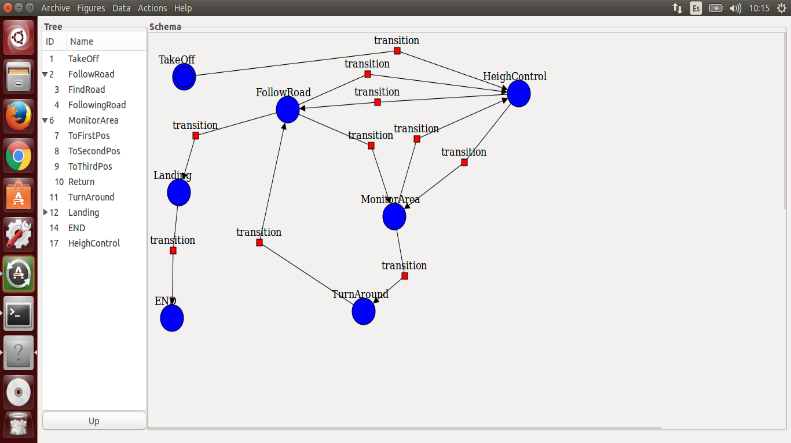
\includegraphics[height=7cm]{imgs/4_visualHFSM5/editor.png}
	\caption{Editor gráfico de VisualHFSM 5.0.}
	\label{fig:editorVisualHFSM}
\end{figure}

Visualmente, el editor gráfico se mantiene igual que en la anterior versión. Sin embargo, aunque no ha habido cambios enormes en la apariencia de la GUI, sí se han realizado distintas modificaciones para mejorar su usabilidad, y se han corregido varios errores del editor que impedían su correcto funcionamiento. \\

%%% Mejora en la navegación por la jerarquía
La modificación principal que hemos realizado al editor gráfico es una mejora de la navegación entre distintos niveles de la jerarquía, de forma que resulte mucho más sencillo cambiar el subautómata seleccionado. Para esto hemos implementado una forma sencilla de navegar hacia los niveles superiores de la jerarquía y una forma rápida de acceder a cualquier subautómata empleando el \textit{Tree View}. \\

Con las versiones anteriores, la forma de visitar el subautómata hijo de un estado era haciendo doble click en dicho estado, pero luego no había forma de volver al subautómata que contenía al estado padre. Para arreglar esto hemos añadido el botón \textit{Up}, que puede verse en la figura \ref{fig:editorVisualHFSM} justo debajo del \textit{Tree View}. Cuando se pulse este botón, los estados y transiciones que se están visualizando en el \textit{Schema View} se ocultan, se busca el subautómata que contiene al estado padre del subautómata actual, y se representan sus estados y transiciones, permitiendo de esta forma volver al nivel superior de la jerarquía. En caso de estar en el subautómata \textit{raíz}, que no tiene ningún padre, el editor simplemente pondrá un mensaje informativo en el terminal indicando que estamos en el subautómata raíz. \\

Además se ha añadido una forma más rápida y sencilla de navegar por los distintos niveles del autómata utilizando el \textit{Tree View}. Para esto, le hemos conectado un manejador a la señal que se emite cuando una fila de nuestro \textit{TreeView} se activa, tal y como se observa en el fragmento de código \ref{lst:connectingSignals}.

\begin{lstlisting}[style=C,caption={conectando un manejador a \texttt{Gtk::TreeView::signal\_row\_activated()}.},label={lst:connectingSignals}]
this->treeview->signal_row_activated().connect(
                 sigc::mem_fun(*this, &VisualHFSM::on_row_activated));
\end{lstlisting}

De esta forma, cada vez que se hace doble click en una fila del \textit{Tree View}, se llama al método \textit{on\_row\_activated}, que puede verse en el fragmento de código \ref{lst:onRowActivated}. Esta función consigue acceder a la fila en la que hemos hecho doble click, y mediante el nombre del estado encuentra el subautómata que lo contiene y lo muestra. De esta forma, se consigue una navegación más dinámica y natural a través de los distintos niveles de la jerarquía. \\

\begin{lstlisting}[style=C,caption={función \texttt{on\_row\_activated}.},label={lst:onRowActivated}]
void VisualHFSM::on_row_activated(const Gtk::TreeModel::Path& path,
                                    Gtk::TreeViewColumn* /* column */){
    Gtk::TreeModel::iterator iter = this->refTreeModel->get_iter(path);

    if (iter){
        Gtk::TreeModel::Row row = *iter;

        std::stringstream name;
        name << row[m_Columns.m_col_name];
        GuiSubautomata* gsub = this->getSubautomataByNodeName(name.str());

        if (gsub == NULL)
            return;

        if (gsub->getId() != this->currentSubautomata->getId()){
            this->currentSubautomata->hideAll();
            this->currentSubautomata = gsub;
            this->currentSubautomata->showAll();
        }
    }else{
        std::cerr << "Couldn't get the row" << std::endl;
    }
}
\end{lstlisting}

%%% Función shutDown() %%%
También hemos añadido la función \textit{shutDown()}, que nos permite finalizar la ejecución del autómata cuando la invocamos. Esto resuelve otra limitación que existía en las versiones anteriores de VisualHFSM, en la que los autómatas nunca terminaban su ejecución, si no que era necesario detener el proceso desde el terminal. Este comportamiento se debe a que los subautómatas se encuentran ejecutándose en un bucle infinito, tal como mostramos en el código a continuación (fragmento de código \ref{lst:loop}).

\begin{lstlisting}[style=C,caption={Ejemplo de un bucle infinito dentro del hilo de un subautómata.},label={lst:loop}]
void* subautomata_1 ( void* ) {
	//variable declaration
	.....

	while (true) {
		gettimeofday(&a, NULL);
		totala = a.tv_sec * 1000000 + a.tv_usec;

		// Evaluation switch
		......

		// Actuation switch
		.....

		//Frecuency Loop Control
		.... 
	}
}
\end{lstlisting}

Aunque esto podría resultar conveniente en algunos casos, definitivamente no lo es siempre, por lo que ahora cuando el generador de código escribe nuestro componente, le añade un \textit{built-in}, la función \textit{shutDown}, que provoca el fin de la ejecución. Para esto, hemos sustituido el \textit{true} de nuestro bucle while por una serie de variables, inicializadas a \textit{true}, de forma que cuando llamamos a la función \textit{shutDown}, cambiará el valor de estas variables a \textit{false}, rompiéndose así el bucle infinito y permitiendo que el código alcance el final sin necesidad de interrumpirlo externamente mediante la consola. \\


%%% Mejora archivo .cfg %%%
Con esta versión de VisualHFSM también hemos mejorado la creación de los archivos de configuración, dotándolos de mayor flexibilidad, de forma que la herramienta es compatible con cualquier robot, real o simulado, cuyas interfaces estén disponibles dentro de la plataforma JdeRobot. Para esto, hemos incluido el campo \textit{Proxy Name}, que permite al usuario elegir este parámetro, como puede observarse en la figura \ref{fig:cfgFileGeneration}. Esto supone una ventaja dado que anteriormente este nombre dependía de la interfaz que se utilizaba. Sin embargo, distintas aplicaciones pueden utilizar diferentes nombres para crear el proxy de una misma interfaz. Esto sucede por ejemplo al utilizar el simulador Gazebo, donde para conectarse a la cámara el \textit{proxy} se llamaba \emph{Camera}, mientras que al utilizar la aplicación \textit{ardrone\_server} para conectarnos al robot real, el nombre que éste recibe es \emph{ardrone\_camera}. Esta modificación permite solventar estas situaciones, haciendo la herramienta completamente compatible con robots simulados y reales, mientras que en las versiones anteriores sería necesario modificar manualmente el archivo de configuración generado para que el componente desarrollado funcionase.

\begin{figure}[htbp]
	\centering
	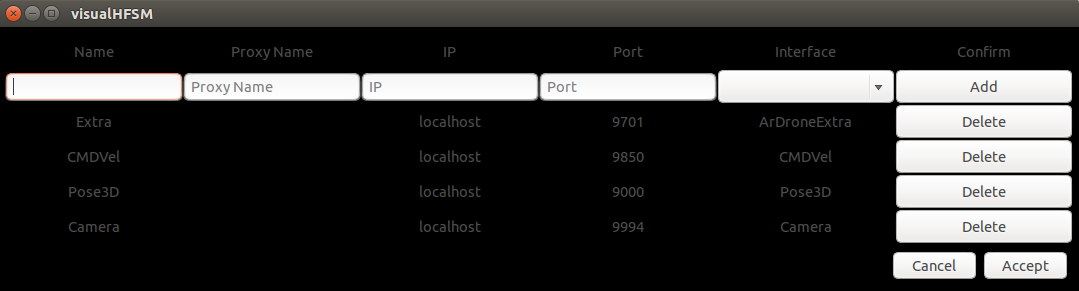
\includegraphics[height=4cm]{imgs/4_visualHFSM5/configFiles.png}
	\caption{Formulario para editar el archivo de configuración.}
	\label{fig:cfgFileGeneration}
\end{figure}


%%% Dependencias resueltas
Otra mejora añadida ha sido resolver las dependencias de la herramienta para permitir ejecutarla desde cualquier directorio. Esta era otra limitación presente en VisualHFSM, dado que sólo podía abrirse desde la carpeta visualHFSM donde estaba todo su código. Esto suponía un problema especialmente porque con la última versión de JdeRobot la instalación puede realizarse mediante paquetes debian sin necesidad de descargarte el código, por lo que para poder utilizar visualHFSM era necesario descargarte el código a parte de GitHub\footnote{\url{https://github.com/RoboticsURJC/JdeRobot/tree/master/src/stable/tools/visualHFSM}}, y compilarlo siguiendo las instrucciones del manual\footnote{\url{http://jderobot.org/index.php/Manual-5\#Installing_JdeRobot_5}}. La razón de que sólo pudiese ejecutarse desde su propia carpeta es que para ejecutar el editor gráfico, necesitaba cargar los distintos archivos \textit{.glade}, tanto del editor como de sus \textit{popups}.  \\

Para solucionar este problema, hemos creado un script para su instalación, \textit{setup.sh}, que aprovechándose de los directorios creados por JdeRobot durante su instalación, copia todos los archivos \textit{.glade} en el directorio \textit{/usr/local/share/jderobot/glade/visualHFSM/}, para los componentes en C++, en \textit{/usr/local/share/jderobot/python/visualHFSM\_py} para los componentes en Python, y en \textit{/usr/local/bin} para el script \textit{getinterfaces.sh}. Con esta nueva distribución, y al cambiar los \textit{paths} de carga de los distintos archivos, conseguimos que el ejecutable de visualHFSM (también situado en \textit{/usr/local/bin}), pueda ejecutarse desde cualquier directorio, dado que sus dependencias estarán instaladas siempre en unas direcciones por defecto. \\


%%% Bug abrir nuevos proyectos
Uno de los errores más molestos que se han solucionado está relacionado con abrir nuevos proyectos cuando estábamos trabajando con otro. El problema era que, al estar trabajando con un proyecto, y abrir otro, el \textit{Tree View} no se limpiaba, sino que pasaba a tener los estados del antiguo proyecto, y del nuevo. Esto, además de ser molesto, creaba problemas en la navegación entre niveles de la jerarquía, dado que aparecían IDs repetidos, que se correspondían a estados no existentes en el proyecto, pero sí en el \textit{Tree View}, lo que podía originar errores al programa. \\


%%% Bug IDs
Por último, otro de los fallos que se han solucionado podía ocasionar que un proyecto quedase inservible, y estaba también relacionado con los IDs. A la hora de crear nuevos estados, transiciones o subautómatas, se les asignaba un ID que debía ser único, que permitía identificarlos. Estos IDs se generaban a partir de 3 variables, como vemos en el código \ref{lst:ids}.

\begin{lstlisting}[style=C,caption={Variables utilizadas para generar los distintos ids.},label={lst:ids}]
class VisualHFSM : public Gtk::Dialog {
	.......
private:
    int id;			// ID for the subautomata created
    idguinode;		// ID for the state created
    idguitransition;// ID for the transition created
    ....
}
\end{lstlisting}

Y dichas variables se incrementaban en uno cuando se creaba un subautómata, estado o transición, respectivamente. El problema aparecía en que, al borrar un estado o subautómata, sus ID también se reducían en uno, pudiendo aparecer así identificadores repetidos que, nuevamente, ocasionaban que la herramienta no funcionase de manera adecuada.


%%%%%%%%%% GUI en ejecución para C++ %%%%%%%%%%
\section{GUI en ejecución para C++}
Como ya hemos comentado en capítulos anteriores, la GUI en ejecución es una característica que visualHFSM tenía en sus primeras versiones y que perdió al dar soporte a autómatas jerárquicos. Esta característica consiste en una GUI de aspecto muy similar a la del editor gráfico, que muestra dinámicamente qué estados están activos durante la ejecución del componente generado por VisualHFSM 5.0. Ésto resulta muy deseable, dado que ahorra mucho tiempo en la depuración al permitir comprobar si el autómata se está comportando como esperamos que haga en tiempo de ejecución, y, en caso de no hacerlo, ver qué es lo que ha pasado y por qué ha podido tener lugar este fallo. La recuperación de esta característica fue el motivo inicial de este TFG.  \\

%%% Explicación general
Para la GUI en ejecución hemos creado la clase \textit{AutomataGui}, que se ejecutará como una aplicación GTK de la clase \textit{Gtk::Application}. Esta clase se importa en el componente creado, se inicializa un objeto, se carga el \textit{glade} y el autómata, y en caso de que todo haya ido bien se ejecutará la GUI en tiempo de ejecución. Si hubiese algún problema durante estos pasos, se notificaría mediante un mensaje en la terminal, pero la ejecución del robot continuaría como si nada hubiese pasado, sin perjudicarle el hecho de que la GUI haya fallado. \\

%%% Como arrancar la GUI
Aunque esta característica es muy conveniente, sólo tiene sentido para depurar, por lo que por defecto el componente se ejecutará sin ella. Esto se debe a que, cuando sepamos que el código funciona como esperamos, y lo ejecutemos en un robot, puede que no estemos interesados en gastar recursos creando un hilo adicional para mostrar la GUI. Por lo tanto, si queremos ejecutar el componente con ella, deberá lanzarse con el argumento \textit{--displaygui=true}, tal como se ve en el ejemplo \ref{lst:executingWithGUI}

\begin{lstlisting}[style=C,caption={Comando para ejecutar un componente C++ con GUI en ejecución.},label={lst:executingWithGUI}]
	monitorArea --Ice.Config=monitorArea.cfg --displaygui=true
\end{lstlisting}

%%% Inicialización
Por lo tanto, al arrancar el componente generado con nuestra herramienta de la forma que acabamos de ver, en primer lugar se leerán los argumentos, y, al encontrar el argumento \textit{--displaygui=true} se pondrá a \textit{true} la variable \textit{displayGui}. A continuación, se conectará a las interfaces ICE que sean necesarias, y después, como \textit{displayGui} es verdad, crea un objeto de la clase \textit{AutomataGui}, pasándole como argumentos los argumentos con los que hemos lanzado el componente, y se llamará a la función \textit{showAutomataGui()}. Esta función se encarga de inicializar el objeto, crear la lista de subautómatas necesaria para su representación gráfica, y si todo ha ido bien, crear un nuevo hilo en el que se ejecutará la aplicación GTK. Esto puede verse en el fragmento de código \ref{lst:initAutomataGui}. \\

\begin{lstlisting}[style=C,caption={Código encargado de inicializar el objeto automatagui.},label={lst:initAutomataGui}]
bool showAutomataGui () {
	if (automatagui->init() < 0){
		std::cerr << "warning: could not show automatagui" << std::endl;
		return false;
	}
	automatagui->setGuiSubautomataList(createGuiSubAutomataList());
	pthread_create(&thr_automatagui, NULL, &runAutomatagui, NULL);
	automatagui->loadGuiSubautomata();
	return true;
}

int main (int argc, char* argv[]) {
	int status;
	Ice::CommunicatorPtr ic;

	try {
		ic = Ice::initialize(argc, argv);
		readArgs(&argc, argv);

		// Create proxys
		.....
		
		if (displayGui){
			automatagui = new AutomataGui(argc, argv);
			displayGui = showAutomataGui();
		}

		//create subautomatas threads
		pthread_create(&thr_sub_1, NULL,
		 &subautomata_1, NULL);

		//join subautomatas threads
		pthread_join(thr_sub_1, NULL);
		if (displayGui)
			pthread_join(thr_automatagui, NULL);
			
	} catch ( const Ice::Exception& ex ) {
		std::cerr << ex << std::endl;
		status = 1;
	} catch ( const char* msg ) {
		std::cerr << msg << std::endl;
		status = 1;
	}

	if (ic)
		ic->destroy();

	return status;
}
\end{lstlisting}

La inicialización se encarga de cargar el archivo \textit{.glade} que contiene la GUI, y de inicializar algunos de sus componentes gráficos como el \textit{Tree View} o el botón \textit{Up}, y de asignar los manejadores a las señales necesarias para poder responder de manera adecuada a los eventos que sucedan en la GUI. \\

Una vez que hemos inicializado nuestro objeto, es necesario crear la lista de subautómatas, con los nodos y transiciones que contiene cada uno para poder representarlos. Aquí nos enfrentamos a un primer problema, dado que, para construir esta lista en el editor gráfico es necesario analizar el archivo XML con el que se está trabajando, pero esto haría que los componentes generados dependiesen del fichero XML, que puede estar en cualquier sitio. Para solucionar esto, nos hemos aprovechado de que el generador de código ya tiene acceso a esta lista de subautómatas, por lo que al generar el componente, le escribe la función \textit{createGuiSubAutomataList()}, de forma que al ejecutarla va creando los subautómatas correspondientes, y les va añadiendo sus estados y transiciones, con las coordenadas en las que deberán pintarse. Para esto, el generador de código se recorre las listas de estados y transiciones de cada subautómata, de forma que sabe qué parámetros tiene que pasarle a los constructores para acabar teniendo la misma lista. Un ejemplo de esta función puede verse en el código de ejemplo \ref{lst:createGuiSubAutomataList}.

\begin{lstlisting}[style=C,caption={Función createGuiSubAutomataList() creada por el generador de código.},label={lst:createGuiSubAutomataList}]
std::list<GuiSubautomata> createGuiSubAutomataList(){
	std::list<GuiSubautomata> guiSubautomataList;
	//Creating the subautomata
	GuiSubautomata* guiSubautomata1 = new GuiSubautomata(1, 0);

	//Creating and adding nodes to this subautomata
	guiSubautomata1->newGuiNode(1, 0, 163, 201);
	guiSubautomata1->setIsInitialLastGuiNode(1);
	guiSubautomata1->setNameLastGuiNode("GO");

	guiSubautomata1->newGuiNode(2, 0, 539, 238);
	guiSubautomata1->setIsInitialLastGuiNode(0);
	guiSubautomata1->setNameLastGuiNode("wait");

	//Creating and adding nodes to this subautomata
	Point* origin11 = new Point(163, 201);
	Point* destiny11 = new Point(539, 238);
	Point* midPoint11 = new Point(357, 116);
	guiSubautomata1->newGuiTransition(*origin11,
					 *destiny11, *midPoint11, 1, 1, 2);

	Point* origin12 = new Point(539, 238);
	Point* destiny12 = new Point(163, 201);
	Point* midPoint12 = new Point(342, 308);
	guiSubautomata1->newGuiTransition(*origin12,
					 *destiny12, *midPoint12, 2, 2, 1);

	guiSubautomataList.push_back(*guiSubautomata1);

	return guiSubautomataList;
}
\end{lstlisting}

%%% Comparación GUIs
Una vez que el objeto \textit{automatagui} ha sido correctamente inicializado, la interfaz gráfica se mostrará en pantalla, tal y como se muestra en la figura \ref{fig:newRuntimeGuiCPP}, donde podemos ver que los estados activos se pintan en verde, tanto en el \textit{Schema View} como en el \textit{Tree View}, en los distintos niveles de la jerarquía. \\
 
\begin{figure}[htbp]
	\centering
	\begin{subfigure}{0.45\textwidth}
	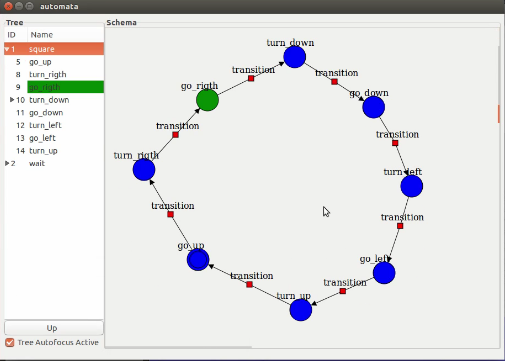
\includegraphics[height=5cm]{imgs/4_visualHFSM5/newRuntimeGuiCPP.png}
	\caption{Nueva GUI en tiempo de ejecución.}
	\label{fig:newRuntimeGuiCPP}
	\end{subfigure}
	\hfill
	\centering
	\begin{subfigure}{0.45\textwidth}
	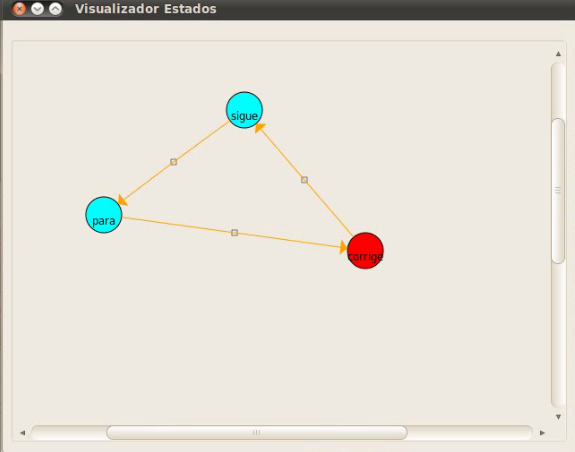
\includegraphics[height=5cm]{imgs/4_visualHFSM5/oldRuntimeGui.png}
	\caption{Antigua GUI en tiempo de ejecución.}
	\label{fig:oldRuntimeGui}
	\end{subfigure}
\caption{Comparación de la nueva y la antigua GUI en tiempo de ejecución.}
\label{oldVsNew}
\end{figure}


Al cargar la GUI por primera vez, cuando se crea un estado se comprueba si es un estado activo. Para esto, tiene que ser el estado inicial de su subautómata, y todos sus padres (en caso de tenerlos), también deben ser el estado inicial. Si esto se cumple, este estado se pintará de verde en el \textit{Schema View} y con el fondo en este mismo color en el \textit{Tree View}. En caso contrario, el estado se pintará de azul en el \textit{Schema View} y se dejará el fondo blanco en el \textit{Tree View}. Con esto se consigue que los primeros nodos activos se representen en la GUI como queremos.  \\

El siguiente paso es que cuando se produce una transición entre estados, se cambien los colores en la GUI para actualizar la representación, pero si la GUI se ejecuta desde un hilo que no sea el principal puede dar problemas y terminar su ejecución. Para arreglar esto, hemos utilizado un objeto \textit{Glib::Dispatcher dispatcher} y la función \textit{notifySetNodeAsActive(std::string nodeName)}. Cuando en un subautómata tiene lugar una transición, en su hilo se llama a esta función con el nombre del nodo que hay que marcar como activo. Esta función introduce el nombre en una cola síncrona, para evitar problemas de condiciones de carrera, y hace que el objeto \textit{dispatcher} emita una señal, que será recogida por un manejador en el hilo de la GUI. Cuando el manejador se activa, extrae el primer nombre que se ha introducido en la cola y busca el subautómata que lo contiene. Entonces, marca como no activado al anterior nodo activo y activa el nuevo estado. En el fragmento de código \ref{lst:notifySetActive} se puede ver el código que se encarga del proceso descrito.

\begin{lstlisting}[style=C,caption={Ejemplo de como se notifica a la GUI que debe cambiar el nodo activo.},label={lst:notifySetActive}]
void AutomataGui::on_notify_received(){

	pthread_mutex_lock(&this->activesNodesNames.lock);
	if (this->activesNodesNames.queue.empty()){
		std::cerr << "ERROR: actives nodes names queue is empty" << std::endl;
		return;
	}
	std::string activeName = this->activesNodesNames.queue.front();
	this->activesNodesNames.queue.pop();
	pthread_mutex_unlock(&this->activesNodesNames.lock);

	GuiSubautomata* subautomata = this->getSubautomataByNodeName(activeName);
	std::string lastActive = subautomata->getActiveNode();
	GuiNode* node;

	node = subautomata->getGuiNode(lastActive);
	this->setNodeAsActive(node, subautomata, false);

	node = subautomata->getGuiNode(activeName);
	this->setNodeAsActive(node, subautomata, true);
}


void AutomataGui::notifySetNodeAsActive(std::string nodeName){
	pthread_mutex_lock(&this->activesNodesNames.lock);
	this->activesNodesNames.queue.push(nodeName);
	pthread_mutex_unlock(&this->activesNodesNames.lock);
	this->dispatcher.emit();
}
\end{lstlisting}

Además, en el fragmento de código \ref{lst:setNodeAsActive} se observa que la función \textit{setNodeAsActive} actualiza el estado el nodo que recibe como argumento, y comprueba si tiene algún hijo, y en caso de tenerlo se llama concurrentemente a sí misma pero pasándole como nodo el nombre de su nodo hijo. De esta forma, se actualiza el estado del nodo y de todos sus hijos.

\begin{lstlisting}[style=C,caption={función setNodeAsActive},label={lst:setNodeAsActive}]
void AutomataGui::setNodeAsActive(GuiNode* node,
								 GuiSubautomata* subautomata, bool active){
	if(active){
		subautomata->setActiveNode(node->getName());
		node->changeColor(ITEM_COLOR_GREEN);
	}else{
		node->changeColor(ITEM_COLOR_BLUE);
	}

	if(!this->setActiveTreeView(node->getName(), 
		active, this->refTreeModel->children()))
 		std::cerr << "NOT FINDED " << node->getName() << std::endl;	

 	int sonId = node->getIdSubautomataSon();
 	if (sonId != 0){
 		GuiSubautomata* subSon = this->getSubautomata(sonId);
 		std::string nodeName = subSon->getActiveNode();
 		GuiNode* nodeAux = subSon->getGuiNode(nodeName);
 		this->setNodeAsActive(nodeAux, subSon, active);
 	}
}
\end{lstlisting}

Por último, en la figura \ref{oldVsNew} podemos ver una comparación de la nueva y la vieja GUI en ejecución. Como se puede observar son completamente distintas, dado que hemos optado por que la apariencia de esta GUI sea lo más similar posible a la del editor gráfico. Además, se le ha añadido el \textit{Tree View}, que permite ver el estado general del autómata, monitorizando que todos los estados activos en toda la jerarquía, no sólo en el nivel actual. \\

%%%%% EJEMPLOS DE VALIDACIÓN
Todas las funcionalidades descritas en este apartado han sido validadas experimentalmente. Para mostrar esto, hemos seleccionado una de las varias aplicaciones que hemos desarrollado utilizando componentes en C++, la aplicación \textit{Cuadrado con un Pioneer}, que será explicada en detalle en el capítulo 5.


%%%%%%%%%% Generación de código Python %%%%%%%%%%
\section{Generación de código en Python}
Otra de las grandes mejoras que tiene VisualHFSM 5.0 frente a otras versiones es que se ha ampliado el generador de código automático de forma que ahora permite generar código en Python también. Esto aumenta en gran medida la flexibilidad y potencia de la herramienta, dado que ahora ofrece soporte para los dos lenguajes, y además, se acerca más a la tendencia de los componentes de JdeRobot, donde los programas en Python son cada vez más habituales. Python es un lenguaje elegante, cómodo y flexible que está teniendo una gran acogida en el mundo de la robótica, que resulta especialmente interesante por los siguientes motivos:

\begin{itemize}
\item Se trata de un lenguaje interpretado, no compilado. Esto resulta increíblemente práctico, y además, en nuestra herramienta ahorra la necesidad de generar un fichero CMake para realizar la compilación, que además tarda algunos minutos. Resulta muy cómodo realizar cambios y probarlos directamente sin necesidad de compilar.
\item Su sintaxis es especialmente clara y directa, lo que hace que sea un lenguaje muy fácilmente legible.
\item Su tiempo de ejecución de sus instrucciones está muy cercano al de programas escritos en C, algo muy importante para la robótica.
\item La gestión de la memoria se hace de forma automática. No resulta necesario la declaración de variables ni liberar espacio.
\item Ofrece tipos de datos de alto nivel como \textit{strings}, tuplas, listas, diccionarios o archivos, entre otros, con una gran variedad de funciones para trabajar con ellos de forma cómoda.
\item Tiene una enorme librería estándar, lo cual añade un gran grado de libertad a la hora de trabajar con este lenguaje.
\end{itemize}

Para generar el código en Python, se ha creado una nueva plantilla donde se empotrará el código de los estados y las transiciones introducido por el desarrollador mediante el editor gráfico, así como el resto de variables y funciones auxiliares que pueda considerar necesarias. Se trata de una plantilla multihilo, en la que se crea un hilo distinto por cada subautómata. Al compararla con la plantilla en C++, se trata de una plantilla mejor organizada, con menos posibilidades de fallos inesperados y un código final más legible. Además, el archivo \textit{.py} generado se creará como un ejecutable, de forma que puede utilizarse del mismo modo que se utilizaban los componentes de C++. \\

La plantilla que se utiliza para generar el código en Python no es la misma que la que se utilizaba en C++, si no que ahora sigue un modelo de programación orientada a objetos, donde todos los datos y funciones del autómata se encuentran dentro de la clase \textit{Autómata}, de forma que la comunicación entre distintos subautómatas es mucho más sencilla, dado que es posible la utilización de elementos de la clase para ello. Además, al usar una plantilla basada en la programación a objetos, conseguimos también la posibilidad de crear clases internas, de forma que el desarrollador cuenta con más herramientas para organizar el código como mejor le parezca, pero manteniendo un alto nivel de abstracción.  \\

Por último, el componente en Python cuenta también con un objeto \textit{threading.Lock()}, por si el código que se va a ejecutar es sensible a las condiciones de carrera. Hay que tener en cuenta para esto que, cada subautómata sigue ejecutándose como un hilo distinto cada uno, por lo que es muy probable que aparezcan condiciones de carrera si se utilizan distintos niveles de jerarquía dentro del autómata. \\

\begin{figure}[htbp]
	\centering
	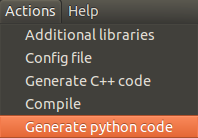
\includegraphics[height=3cm]{imgs/4_visualHFSM5/generatePythonCode.png}
	\caption{Menú con la opción de generar codigo Python.}
	\label{fig:pythonCodeGenerator}
\end{figure}


%EXPLICACION SENCILLA DEL LA PLANTILLA
Al generar el código la plantilla se va completando dinámicamente en función a la información introducida con el editor gráfico. En resumen, para este proceso se generan las cabeceras que importan todas las librerías necesarias, tanto por defecto como las introducidas por el usuario. Entonces, se genera la clase autómata, donde se definen todas las variables y funciones que el usuario haya introducido. Adicionalmente, se generan las funciones de los subautómatas, una por cada subautómata existente. Dichas funciones serán ejecutadas cada una en un hilo distinto y se encargan de revisar si toca transitar a otro estado, y de ejecutar el código correspondiente en caso de ser necesario. Después se crea la función encargada de que los subautómatas comiencen su ejecución, la función encargada de esperar a que terminen, la función responsable de conectarse al robot y la función \texttt{shutDown()}, que terminará la ejecución en caso de que sea llamada. Por último, fuera de la clase autómata, se genera el cuerpo del \texttt{main}, que será llamado cuando ejecutemos el componente generado y se encargará de llamar a las funciones encargadas de conectarse al robot, empezar la ejecución de los distintos subautómatas y quedarse esperando a que estos hilos finalicen. \\


%%% Descripción del generador de código
A continuación abordaremos este proceso en detalle. Cuando el autómata está preparado, al hacer click en el menú \textit{Actions} a la opción de \textit{Generate Python code}, tal y como se ve en la figura \ref{fig:pythonCodeGenerator}, se activa su manejador, la función \textit{on\_menubar\_clicked\_generate\_python\_code}. Esta función se encarga de analizar el último archivo XML guardado del proyecto mediante un objeto \textit{SaxParser}, preparar la cadena con la ruta al archivo XML y prepararlo para generar la ruta para el archivo Python y el archivo de configuración para ICE, y cuando ha terminado con esto, crea un objeto generador de código y llama a la función \texttt{init\_py()}. \\

\begin{lstlisting}[style=python,caption={Función \texttt{init\_py()} del generador de código.},label={lst:initPy}]
int Generate::init\_py (){
	this->fs.open(this->path.c_str(), std::fstream::out);
	if (this->fs.is_open()){
		this->generateHeaders_py();
		this->generateAutomataClass_py();
		this->generateMain_py();
		this->fs.close();

		this->fs.open(this->cfgpath.c_str(), std::fstream::out);
		if (this->fs.is_open()){
			this->generateCfg();
			this->fs.close();
		}

		std::string permission("chmod +x " + this->path);
		system(permission.c_str());
		return 0;
	}else{
		return -1;
	}
}
\end{lstlisting}

Como podemos observar, la función que vemos en el fragmento de código \ref{lst:initPy} es la encargada de escribir todo el código del componente y su archivo de configuración, así como de otorgarle permisos de ejecución. Para esto sigue los siguientes pasos:

\begin{enumerate}
\item Abrir el fichero en el que se va a escribir el código, cuya ruta se le ha pasado al constructor de la clase \textit{Generate} como argumento. A continuación comprueba que el fichero se haya abierto correctamente, devolviendo -1 para notificar que ha habido un error en caso contrario.
\item La función \texttt{generateHeaders\_py} se encarga de escribir \texttt{\#!/usr/bin/python} para que cuando el código sea un ejecutable sea interpretado por el intérprete de Python y se encarga de realizar los \texttt{imports} necesarios. Para esto, importa las librerías adicionales que se le han añadido mediante el editor, las interfaces de JdeRobot que se van a utilizar para conectarse a los sensores y actuadores, y algunas otras librerías necesarias como \texttt{sys}, \texttt{signal} o la clase \texttt{AutomataGui} del módulo \texttt{automatagui}, entre otros.
\item \texttt{generateAutomataClass\_py} se encarga de escribir toda la información relativa al autómata.
\item A continuación la función \texttt{generateMain\_py} se encarga de generar el cuerpo del main. Esto es el código que será ejecutado cuando se ejecute el componente.
\item Tras generar el cuerpo del \texttt{main}, y se abre otro nuevo para escribir el archivo de configuración. De esto se encarga la función \texttt{generateCfg()}, que es la misma que ya existía en el generador de código C++.
\item Por último, cuando todo el código ha sido generado, la función le da permisos de ejecución para que pueda ejecutarse como un script, sin necesidad de llamar al intérprete Python por la línea de comandos.
\end{enumerate}

\begin{lstlisting}[style=python,caption={Función \texttt{generateAutomataClass\_py()}.},label={lst:generateAutomataClass}]
void Generate::generateAutomataClass_py(){
	this->fs << "class Automata():" << std::endl;
	this->fs << std::endl;
	this->generateAutomataInit_py();
	this->generateFunctions_py();
	this->generateStartThreads_py();
	this->generateCreateGuiSubautomataList_py();
	this->generateShutDown_py();
	this->generateRunGui_py();
	this->generateSubautomatas_py();
	this->generateConnectToProxys_py();
	this->generateDestroyIc_py();
	this->generateStart_py();
	this->generateJoin_py();
	this->generateReadArgs_py();
}
\end{lstlisting}

Como se puede deducir de la explicación anterior, la función responsable de generar casi todo el código del autómata es \textit{generateAutomataClass\_py}, la cual puede verse en el código \ref{lst:generateAutomataClass}. Esta función también se basa en otras funciones secundarias para realizar el trabajo de una forma más organizada y legible. En primer lugar, \textit{generateAutomataInit\_py()} se encarga de escribir el constructor, donde se inicializa el \textit{lock} para ese autómata, la variable \textit{self.displayGui} con valor \textit{False} por defecto, los \textit{arrays} con los distintos estados de cada subautómata y las variables donde se guarda el estado actual en el que se encuentra cada autómata así como las variables que controlan si se sigue entrando en el bucle de ejecución. Podemos ver un ejemplo de constructor creada por esta función en \ref{lst:initExample}.

\begin{lstlisting}[style=python,caption={Ejemplo de constructor creado por el generador de código},label={lst:initExample}]

	def __init__(self):
		self.lock = threading.Lock()
		self.displayGui = False
		self.StatesSub1 = [
			"PingPong",
			"Numbers",
		]

		self.StatesSub3 = [
			"Ping",
			"Ping_ghost",
			"Pong",
			"Pong_ghost",
		]

		self.StatesSub4 = [
			"1",
			"1_ghost",
			"2",
			"2_ghost",
			"3",
			"3_ghost",
		]

		self.StatesSub5 = [
			"wait2",
			"wait2_ghost",
			"wait1",
			"wait1_ghost",
		]

		self.sub1 = "Numbers"
		self.run1 = True
		self.sub3 = "Ping_ghost"
		self.run3 = True
		self.sub4 = "1_ghost"
		self.run4 = True
		self.sub5 = "wait1_ghost"
		self.run5 = True
\end{lstlisting}

Una vez que se ha generado la función \texttt{init}, se escriben las funciones que el usuario ha creado mediante el editor gráfico (en caso de haberlas), y la función \textit{startThreads()}, que será llamada para empezar los hilos de los distintos subautómatas. A continuación se escribirá la función \textit{shutDown()}, que funciona igual que en el componente C++, la función que permite generar la lista de subautómatas necesaria para la GUI en tiempo de ejecución. Después se generan las funciones que llamarán los hilos de los subautómatas, con todas sus variables, su \texttt{if} de evaluación y su \texttt{if} de actuación, dado que en Python no existen los \textit{switch}, escribiendo entonces la función que se encargará de comunicarse con los sensores y actuadores usando ICE y la función para eliminar el objeto ICE al terminar la ejecución. Por último se generará la función encargada de iniciar la GUI en tiempo de ejecución, la función que se llamará para esperar a que los hilos terminen y la \textit{readArgs()}, encargada de leer los argumentos de entrada. \\

Para terminar con esta sección, comentaremos cómo es el generador del \texttt{main}, que puede verse en el fragmento de código \ref{lst:mainExample}. En este caso, el \texttt{main} generado es igual para todos los autómatas, dado que lo que varía es el contenido de las funciones que llama. Comparándolo con el \texttt{main} de los componentes de C++ se trata de un \texttt{main} más compacto y legible, dado que toda la funcionalidad ha sido organizada en funciones que se encargan de realizar el trabajo necesario. \\

\begin{lstlisting}[style=python,caption={Función encargada de generar el cuerpo del programa en Python.},label={lst:mainExample}]

void Generate::generateMain_py (){
	this->fs <<
"if __name__ == '__main__':\n\
	signal.signal(signal.SIGINT, signal.SIG_DFL)\n\
	automata = Automata()\n\
	try:\n\
		automata.connectToProxys()\n\
		automata.readArgs()\n";

	this->fs.flush();
	this->fs <<
"		automata.start()\n\
		automata.join()\n\n\
		sys.exit(0)\n\
	except:\n\
		traceback.print_exc()\n\
		automata.destroyIc()\n\
		sys.exit(-1)\n";
}
\end{lstlisting}


%%%%%%%%%% GUI en ejecución para Python %%%%%%%%
\section{GUI en ejecución para Python}
Al igual que sucede con los componentes generados en C++, los componentes escritos en Python también disponen de una GUI en tiempo de ejecución para depurar. En este caso no se ha utilizado GTK, si no que en su lugar se ha optado por realizarla utilizando Qt, a través de su \textit{binding} para Python: \textit{PyQt}, en su versión 4, tal y cómo explicamos en el capítulo 3 de esta memoria.

\begin{figure}[htbp]
	\centering
	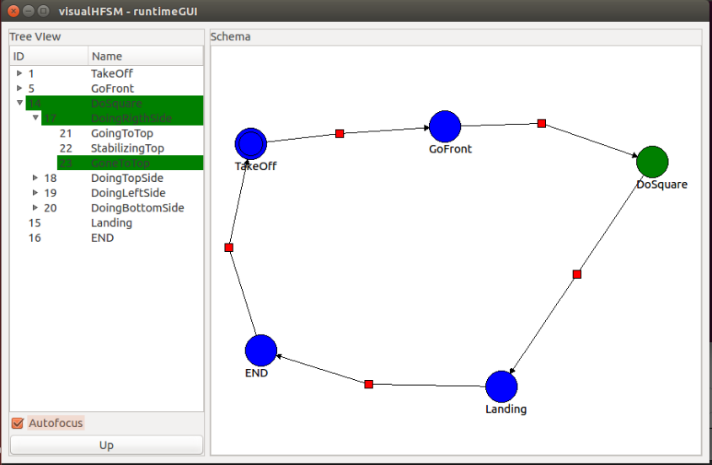
\includegraphics[height=5cm]{imgs/4_visualHFSM5/runtime.png}
	\caption{GUI en tiempo de ejecución con "Autofocus" activo.}
	\label{fig:runtimeGUIPython}
\end{figure}

Sin embargo, a pesar de utilizar lenguajes y bibliotecas gráficas diferentes la funcionalidad básica que ofrece es la misma: mostrar dinámicamente que estados se encuentran activos para facilitar la depuración. También hemos intentado que el aspecto de la interfaz sea lo más similar posible al que utiliza el componente en C++, tal y como se aprecia en la figura \ref{fig:runtimeGUIPython}. Además, esta interfaz gráfica también viene desactivada por defecto, y si se quiere activar es necesario ejecutar el componente con el argumento \textit{--displaygui=true}, igual que sucedía con el componente en C++, tal y como observamos en el ejemplo \ref{lst:executingWithGUIPython}. \\

\begin{lstlisting}[style=C,caption={Comando para lanzar un componente python con GUI en ejecución.},label={lst:executingWithGUIPython}]
	monitorArea.py --Ice.Config=monitorArea.cfg --displaygui=true
\end{lstlisting}

Pero no sólo el aspecto y la forma de activarla son similares, si no que el cómo funciona también es bastante parecido. El encargado de mostrar y actualizar la GUI sigue siendo un objeto de la clase \textit{Automata()}. El generar la GUI tampoco depende del archivo XML, si no que el generador de código crea una función para reconstruir la lista de subautómatas reduciendo así las dependencias con otros ficheros al mínimo, y el mecanismo para representar los estados activos es en esencia el mismo. También es el hilo de la GUI el responsable de actualizar los estados activos, para asegurar el correcto funcionamiento de la aplicación y evitar problemas por culpa del multihilo. \\

Sin embargo, existen algunas diferencias respecto a cómo se lleva a cabo el proceso de notificar al hilo de la GUI que tiene que actualizar sus estados activos. En esta ocasión no necesitamos utilizar un objeto \textit{Dispatcher} para emitir la señal, si no que como muestra en el fragmento \ref{lst:qtSignal}, hemos creado una señal utilizando el módulo \textit{QtCore} de Qt, de forma que la señal puede llevar también el nombre del estado, ahorrándonos así la necesidad de utilizar una cola.

\begin{lstlisting}[style=python,caption={Creación de señal con Qt.},label={lst:qtSignal}]
activeNodeSignal = QtCore.pyqtSignal(str)
\end{lstlisting}

%%% NECESARIO???? 
En resumen, cuando se produce una transición el subautómata enviará la señal \texttt{activeNodeSignal} con el nombre del nuevo estado. Esta señal será recogida por el hilo de la GUI en ejecución, que se encargará de actualizar la información que muestra. \\

Viendo esto más detenidamente, cuando se produce una transición en un subautómata, éste llama a la función \textit{notifySetNodeAsActive(nodeName)} que envía la señal que acabamos de comentar. Entonces, en el hilo de la GUI se activará el manejador asignado para esta señal, activándose la función \textit{notifySetNodeAsActiveReceived(nodeName)}. Y a partir de este punto el proceso tiene lugar igual que en el componente de C++. En primer lugar se marca el anterior nodo activo como inactivo y se marca el nuevo como activo. Esto se realiza mediante la función \textit{setNodeAsActive}, que se encarga de cambiar el estado del nodo y de todos los que cuelgan de él. En el ejemplo \ref{lst:stateActivationPython} podemos observar las funciones encargadas de emitir y recibir la señal que hemos explicado.

\begin{lstlisting}[style=python,caption={Activación de estados en Python.},label={lst:stateActivationPython}]
	def notifySetNodeAsActiveReceived(self, nodeName):
		subAux = self.getSubautomataWithNode(nodeName)
		nodeAux = subAux.getNodeByName(subAux.getActiveNode())		

		if nodeAux != None:
			self.setNodeAsActive(nodeAux, subAux, False)

		nodeAux = subAux.getNodeByName(nodeName)
		self.setNodeAsActive(nodeAux, subAux, True)


	def notifySetNodeAsActive(self, nodeName):
		self.activeNodeSignal.emit(nodeName)
\end{lstlisting}

En cuanto a la navegación por los distintos niveles de la jerarquía, tanto la GUI en Python como en C++ funcionan igual que el editor gráfico, permitiendo la navegación utilizando el \textit{Tree View}, o bien haciendo doble click en cualquier estados para acceder a sus subautómatas hijos, en caso de tenerlos. Además, las GUI en ejecución disponen de una funcionalidad que no se encuentra disponible en el editor gráfico, y es la opción que hemos llamado \textit{Autofocus}. Esta opción puede activarse mediante el \textit{check box} situado bajo el \textit{Tree View} en la GUI, tal y cómo se ve en la figura \ref{fig:runtimeGUIPython}, y se encarga de expandir automáticamente todos los niveles activos de la jerarquía y colapsar los demás. Esto resulta especialmente útil en autómatas complejos con muchos estados y varios niveles de jerarquía, dado que permite ver todos los estados activos en los distintos niveles de la jerarquía.  \\

Como podemos observar en el fragmento de código \ref{lst:treeViewAutofocus}, cuando activamos la funcionalidad primero comprobamos si el nivel de jerarquía a expandir está ya expandido, y si no lo está comprobamos que la última rama que expandimos, almacenada en la variable \textit{lastExpanded}, no fuese nuestro padre, colapsándola si no lo era. Esto es así para evitar estar expandiendo y contrayendo las distintas ramas sin necesidad. Por último, expandimos el nivel que queríamos y actualizamos la variable \textit{lastExpanded} con la rama que acabamos de expandir. \\

\begin{lstlisting}[style=python,caption={treeViewAutoFocus},label={lst:treeViewAutofocus}]
	def treeViewAutoFocus(self, index):	
		if not self.treeView.isExpanded(index.parent()):
			if not self.lastExpandedIsFather(index):
				self.treeView.collapse(self.lastExpanded)

			if index.parent().isValid():
				self.treeView.expand(index.parent())
		self.lastExpanded = index.parent()
\end{lstlisting}

Por último, la GUI en tiempo de ejecución del componente escrito en Python tiene una funcionalidad que no tienen los componentes en C++, y es que permiten abrir ventanas adicionales para ver otros subautómatas, además del que se muestra en el \textit{Schema View}. Esto puede verse en la figura \ref{fig:multipleSubautomatasGUI} y resulta especialmente útil cuando se quiera observar cómo se comporta el robot en distintos niveles de la jerarquía. Para esto, cada vez que se muestra una ventana nueva se crea un nuevo hilo y se almacena en un \textit{array}. Cuando se cierra se detiene su hilo de ejecución y se elimina de este \textit{array} para que no ocupe espacio. \\

\begin{figure}[htbp]
	\centering
	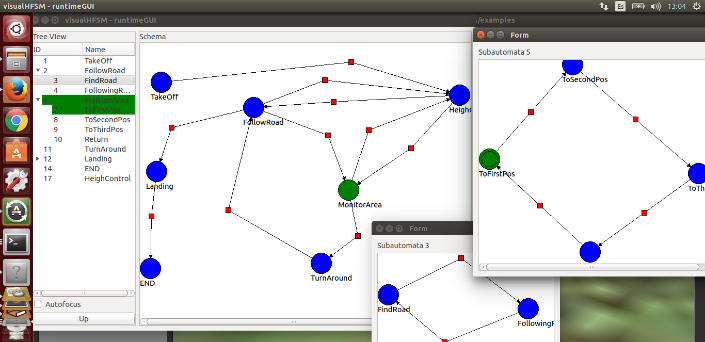
\includegraphics[height=5cm]{imgs/4_visualHFSM5/runtime-hierarchy.png}
	\caption{Multiples subautómatas en ejecución.}
	\label{fig:multipleSubautomatasGUI}
\end{figure}


%%%%%%%%%% Difusión %%%%%%%%%%%
\section{Difusión}
Una vez que hemos alcanzado una versión lo suficientemente madura de VisualHFSM 5.0, nos hemos centrado en darla a conocer para cumplir nuestro cuarto objetivo principal: convertirla en una herramienta utilizada por terceros. \\

Para conseguir esto, empezamos por elaborar una documentación sólida y detallada que explica cómo funciona VisualHFSM y las ventajas que ofrece, que puede encontrarse dentro de la página de JdeRobot\footnote{\url{http://jderobot.org/VisualHFSM}}. Esta documentación incluye:

\begin{itemize}
\item La entrada oficial de la herramienta dentro del manual de JdeRobot\footnote{\url{http://jderobot.org/Tools\#VisualHFSM}}, con una descripción básica, una explicación de su estructura y los detalles de cómo instalarla.
\item Un aviso de que la GUI en tiempo de ejecución está desactivada por defecto y una explicación de cómo ejecutar VisualHFSM si queremos ver esta GUI.
\item Una explicación detallada de cómo utilizar toda la funcionalidad que ofrece la herramienta, separando el editor gráfico, los componentes generados en C++ y los componentes generados en Python.
\item Un vídeo de ejemplo de un componente generado por la herramienta en ejecución, con un enlace a \textit{Running JdeRobot}\footnote{\url{http://jderobot.org/Running_JdeRobot\#VisualHFSM}}, dónde se explica detalladamente cómo ejecutar el ejemplo para poder probarlo.
\end{itemize}

Además, con el fin de dar a conocer VisualHFSM a la comunidad robótica, hemos escrito un artículo\cite{rey2016visualhfsm} al congreso robótico WAF\footnote{\url{http://waf2016.uma.es/}} (\textit{Workshop de Agentes Físicos}), explicando todas las novedades y ventajas que ofrece VisualHFSM 5.0. Este artículo ha sido aceptado y publicado en la edición del WAF de este año. Esto demuestra que la herramienta se centra en un tema que interesa a la comunidad robótica, y contamos con que llame la atención de futuros usuarios. \\

Por último, hemos introducido una práctica preparada para resolverla con VisualHFSM dentro del entorno docente de JdeRobot, \textit{Teaching Robotics}\footnote{\url{http://jderobot.org/Teaching_robotics_with_JdeRobot}}, que cuenta con una serie de prácticas distintas que se utilizan con fines didácticos en los cursos de JdeRobot y en las clases de róbotica de la Universidad Rey Juan Carlos. Al introducir una práctica basada en VisualHFSM damos la oportunidad a los alumnos de robótica de la universidad de futuros cursos a que utilicen la herramienta y aprendan a programar la inteligencia del robot en términos de estados y transiciones de una forma sencilla e intuitiva.

\vspace{1.5cm}
En este capítulo hemos descrito las distintas mejoras que aporta VisualHFSM 5.0 frente a las versiones anteriores y cómo éstas han sido implementadas. En el siguiente capítulo, expondremos varios casos de uso que validan estas mejoras.